%************************************************
\chapter{Class diagrams}\label{ch:class_diagrams} % $\mathbb{ZNR}$
%************************************************

The class diagrams are provided on a per-package level:

\section{View}

The view is connected to a presenter (holds locations that can be changed) and to the model (implements an observer pattern to notify the view about changes.

\begin{figure}[H]
\begin{center}
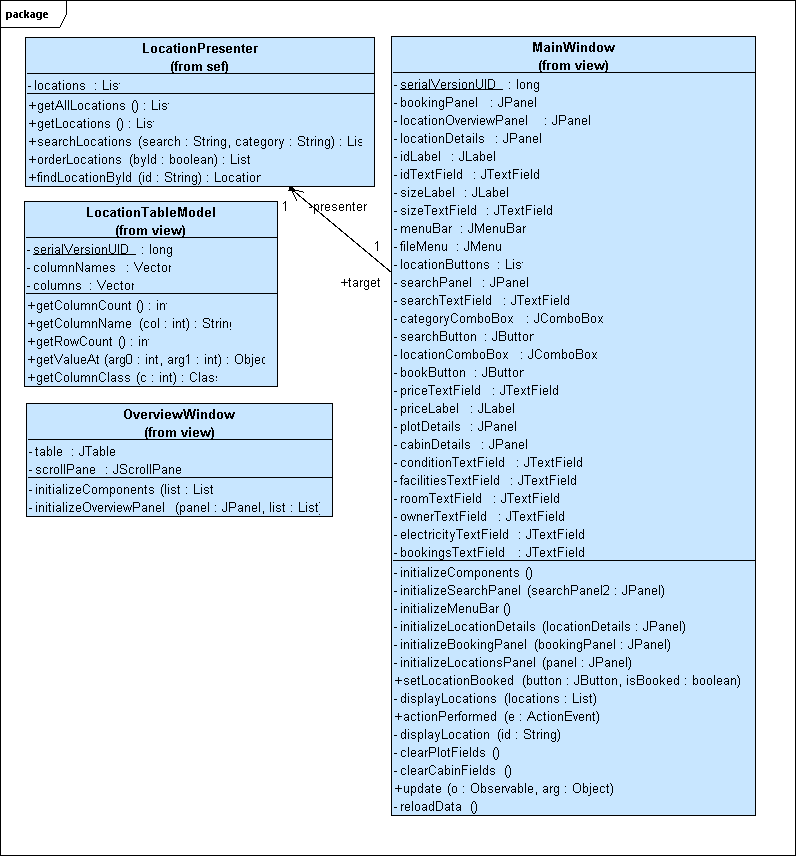
\includegraphics[width=\textwidth]{gfx/class_view.png} 
\end{center}
\caption{Class diagram view package.}
\label{fig:view}
\end{figure}

\section{Model}

\begin{landscape}
\begin{figure}
\begin{center}
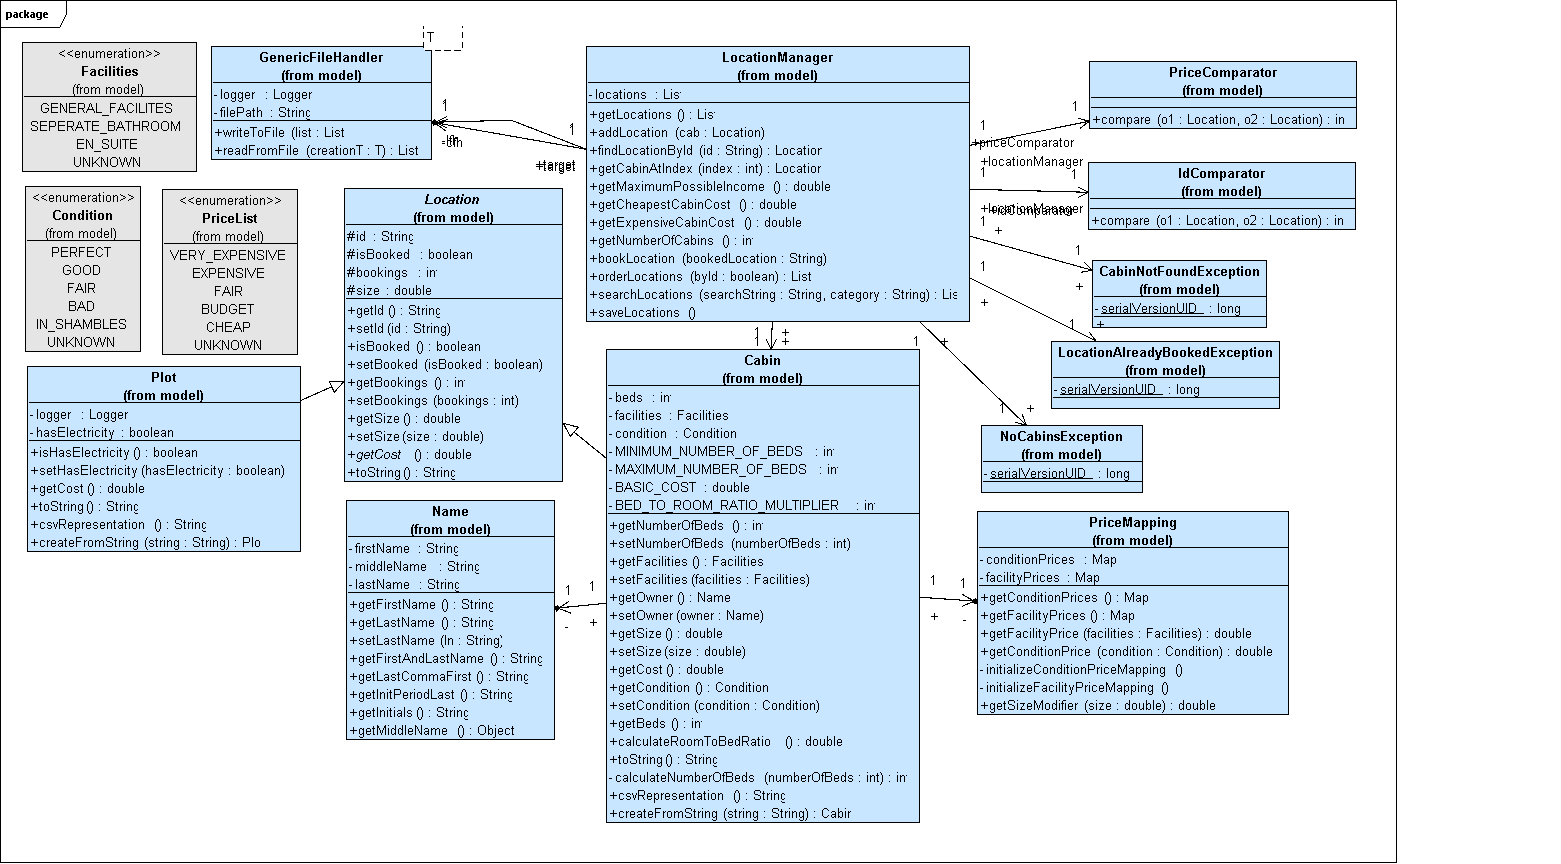
\includegraphics[height=1.00\textheight]{gfx/class_model.png} 
\end{center}
\caption{Class diagram model package.}
\label{fig:model}
\end{figure}
\end{landscape}

\section{Model.Interfaces}

\begin{figure}[H]
\begin{center}
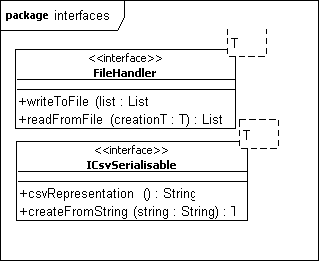
\includegraphics[scale=1]{gfx/class_interfaces.png} 
\end{center}
\caption{Class diagram model.interfaces package.}
\label{fig:model_interfaces}
\end{figure}